\chapter{The Interaction the Stellar Magnetic Cycle with Hall Dead Zones in Protoplanetary Disks}
\label{hall}





\section{Abstract}
We present modeling of a new mechanism for episodic accretion events in protoplanetary disks and demonstrate that this mechanism is able to produce events that would appear similar to observed EXor outbursts.  In the inner disk, a Hall-effect dominated dead zone (region of low turbulence and accretion velocity) is expected to exist.  These dead zones have been shown to exhibit a dichotomous behaviour depending on the sign of the net vertical magnetic field in the disk relative to the spin axis -- they are rather active for an aligned field and dead for an anti-aligned field.  We show that stellar magnetic field contributed to the disk at the inner edge (~0.01 to 0.1 AU) is able to diffuse outward to trigger bursts of accretion from these dead zones on the scale of a few AU.  We model this mechanism in 1 dimension by self-consistently evolving the surface density and net magnetic field in time.  We use this model to calculate light curves and simple black body spectra (as a function of time) for these events. 




\newpage
\section{Introduction}
The interaction between the stellar magnetosphere and accretion disk around a young star has been considered in several contexts.  One context that has not been well explored is the effect of the stellar dipole contribution to the net-field within the disk.  This is important as several recent studies have shown that the presence net vertical field in an accretion disk can enhance the MRI and drive faster accretion.  In addition, the alignment of the net field has been shown to have an interesting interaction with a Hall Dead Zone.   

Observational evidence shows that many young stellar objects (YSOs) undergo bursts of accretion during which the their optical luminosity and total accretion rate can increase by orders of magnitude \citep{herbig77, hartmann96}.  

Historically, these events have been placed into two categories: FU Orionis objects (FUors) and EX Lupi objects (EXors) \citep{herbig89}.  FUors outbursts generally occur for several to tens of years with amplitudes of a few orders of magnitude over the quiescent state, although properties of individual objects vary greatly.  In contrast, EXor outbursts are shorter and weaker, typically bursting for months to years.  They also occur more frequently, typically having a few years between bursts.   

Recently, the distinction between the two cases has become less clear.  Several observations of 'in between' events have led to the idea that these events may be part of a continuous spectrum instead of a dichotomy. 

Many mechanisms have been proposed to explain ...

Non-ideal MHD effects have been shown to play an important role in understanding protoplanetary disk phenomena, with different non-ideal effects dominating in different regions of the disk.  In general, these effects can allow the magnetic field to decouple from the gas such that the magnetorotational instability (MRI) is no longer able to drive turbulence.  These regions of little to no turbulence are generally referred to as "dead zones".  

Dead zones dominated by the Hall Effect are thought to exist in the inner region of the disk ($\leq 1$ AU), and have been shown by several studies to have an interesting behaviour with respect to direction of the vertical magnetic field.  When the field is aligned with the spin axis, the Hall Effect doesn't change the behaviour of the MRI very much, and turbulence is still generated ($\alpha \sim 10^{-2}$).  However, when the vertical field is anti-aligned with the spin of the disk the Hall Effect suppresses the MRI and the dead zone is true to it's name ($\alpha \sim 4*10^{-4}$).

Armitage 2016 suggests that this dichotomous behaviour of hall dead zones could lead to episodic accretion.  While the field is aligned with the spin, the dead zone will be "active", and the turbulence will drive a relatively high accretion rate.  While the field is anti-aligned, the dead zone will be "dead", and the lack of turbulence will cause the accretion rate to be much lower.  Armitage proposes that this change in net-field direction could be caused by the stellar magnetic field diffusing though the inner disk, with the stellar field changing sign on some characteristic timescale, as we have observed for the sun and other stars.  

In this paper we develop a 1D, time-dependent model to explore the viability of this mechanism to produce episodic accretion events, characterize the events that should occur, and briefly compare the results of our modeling to observations.  

The paper is organized as follows: In section 2 we describe the model that we will use.  In section 3 we describe the numerical methods we use to descritize the model and evolve it in time.  In section 4 we describe the initial conditions used and the quiescent state of a disk with a dead zone.  In section 5 we describe the influence of the stellar magnetic field on the disk.  In section 6 we demonstrate simple cases of Hall dead zone behaviour. In section 7 we quantitatively show the characteristics of the episodic accretion events that this mechanism can produce.  In section 8 we compare our modeling to observations of episodic accretion events and speculate as to how these events would fit into the FUors/EXors paradigm.  In Section 9, we summarize our results.  




\newpage
\section{The Model}
\label{1dmodel}
We develop a model using a mean-field approach that self-consistently evolves the net magnetic field and surface density of a turbulent accretion disc.     


\subsection{Static Equations} 
Here we will give and briefly justify the equations that we will use to solve for the state of the disk at any given point in time (SS74-ish, Phil's text).

The sound speed is given by
\begin{equation} 
c_s^2        = \frac{k_b}{\mu m_p}T_c ,              
\end{equation}
where $T_c$ is the temperature at the mid-plane of the disk.  Assuming hydrostatic equilibrium, the vertical pressure scale-height of the disk is determined by balancing the vertical component of the central star's gravity and the vertical pressure gradient.  For a non-self-gravitating disk, the scale height is given by     
\begin{equation} 
h            = \frac{c_s}{\Omega},  
\end{equation}
where $\Omega$ is the angular orbital velocity.

The turbulence in the disk gives rise to an effective viscosity $\nu$, which we will parametrize with the usual $\alpha$-model 
\begin{equation} 
\nu          = \alpha c_s h                    
\end{equation}
where $\alpha$ is a dimensionless parameter that describes the level of turbulence.  This viscosity allows angular momentum to be transported within the disk such that some gas looses angular momentum and accretes inward.  The accretion rate is given by $\dot{m}$ and is related to the viscosity via
\begin{equation} 
\nu \Sigma   = \frac{\dot{m}}{3\pi}
\end{equation}
where $\Sigma$ is the surface density. This accretion dissipates energy.  We will assume that all of this enegy is generated at the mid-plane of the disk, travels through the optically thick disk with optical depth $\tau$, and is radiated from the surface.  The surface temperature $T_d$ and central temperature $T_c$ are then given by
\begin{equation} 
\sigma T_d^4 = \frac{9}{8} \nu \Sigma \Omega^2,
\end{equation} 
\begin{equation} 
T_c^4        = \frac{3}{4} \tau T_{d}. 
\end{equation} 
The optical depth is given by 
\begin{equation} 
\tau         = \frac{1}{2} \Sigma \kappa_R     
\end{equation} 
where $\kappa_R$ is the mean opacity.  $\kappa_R$ will (very generally) be some function of the average gas density $\rho$ and $T_c$:
\begin{equation} 
\kappa_R = \text{power law of } \rho \text{ and } T_c.
\end{equation}
Lastly, $\rho$ can be written as
\begin{equation} 
\rho         = \frac{1}{\sqrt{2\pi}} \frac{\Sigma}{h}.
\end{equation}
Equations 1-9 form a system of 9 equations and 9 unknowns: $c_s, T_c, h, \nu, \Sigma, T_d, \tau, \kappa_R, \rho$.  If $\alpha$ and $\dot{m}$ can be specified a-priori and $\kappa_R$ is given by a power law of $\rho$ and $T_c$, these equations have analytic solutions and the system can be solved self-consistently.  This is, essentially, the familiar problem solved by \cite{shakura73}.  


\subsection{Coupling MRI Turbulence to the Net Magnetic Field } 
For a disk with a Hall-effect-dominated dead zone, the turbulence in the disk is coupled to the net magnetic field.  Non-ideal MHD simulations of the MRI of this case have shown that the space-time averaged $\alpha$ value in the case of a net field aligned with the spin axis is $\sim 0.01$ to $0.1$.  However, in the case that the field is anti-aligned with the spin axis the MRI is suppressed more significantly and $\alpha \sim 4 \times 10^{-4}$.  

We will model this behaviour in two different ways.  The first and simpler, taking the above statement to be strictly true:
$$
\alpha=
\begin{cases}
~10^{-2}, \ \ \ \ \ \ \beta_z \cdot \Omega > 0  \\
~4 \cdot 10^{-4}, \ \ \beta_z \cdot \Omega < 0
\end{cases}
$$

We will also consider the likely more physical case where $\beta$ must cross some threshold in order to...

We will use these relationships, to couple the field to the turbulence and therefore the surface density evolution.   


\subsection{Surface Density Evolution} 
\label{sdEvo}
The surface density profile of the disk is evolved using the usual equation for a thin Keplerian disk evolving due to viscous torques:
\begin{equation}
v\frac{\partial \Sigma}{\partial t} = 
\frac{3}{r} \frac{\partial}{\partial r} \bigg[
	r^{1/2} \frac{\partial}{\partial r} \Big( 
		r^{1/2} \nu \Sigma
	\Big)
\bigg],
\end{equation}
where $\Sigma$ is the surface density.  


\subsection{Net Magnetic Field Evolution} 
\label{bEvo}
We will follow \cite{lubow93} to time-evolve the poloidal and radial components of the magnetic field in a turbulent disc.  The magnetic potential $\psi$ is defined by 
\begin{equation}
B_z = \frac{1}{r} \frac{\partial \psi}{\partial r} 
\end{equation}
\noindent where $B_z$ is the vertical component of the net magnetic field.  The potential's time evolution is given by  
\begin{equation}
\frac{\partial \psi }{\partial t} = -r(v_{\text{adv}}B_z + v_{\text{diff}} B_{rs}) 
\end{equation}
where $B_{rs}$ is the radial magnetic at the surface of the disc, $v_{\text{adv}}$ is the advective velocity, and $v_{\text{diff}}$ is the diffusive velocity.  Given $\psi$, $B_{rs}$ can be determined by solving an integral equation, or equivalently solving a linear system of equations in the case of the discretized problem.  (Need to insert a little more here) 

Following the $\alpha$ model of turbulence, the advective velocity and time-scale are given by 
\begin{equation}
v_{\text{adv}}=\frac{-3}{2} \frac{\nu}{r}, \tau_{\text{adv}}=\frac{r}{v_{\text{adv}}}. 
\end{equation}
 
The turbulent magnetic diffusivity $\eta$ is defined by assuming a constant magnetic prandtl number $Pr=\frac{\nu}{\eta}$ (expected to be order unity).  The diffusive speed and time-scale are then given by   
\begin{equation}
v_{\text{diff}}=\frac{\eta}{h} = \frac{\eta}{r} \Big(\frac{h}{r}\Big)^{-1}, \tau_{\text{diff}}=\frac{r}{v_{\text{diff}}}. 
\end{equation}

In this case, the relevant dimensionless parameter that describes the ratio of viscous diffusion to magnetic diffusion is the effective prandtl number 
\begin{equation}
Pr_{\text{eff}} = \frac{v_{\text{adv}}}{v_{\text{diff}}} = \frac{3}{2} \frac{h}{r}Pr.
\end{equation} 
Note that diffusion is faster than advection by a factor of $(h/r)^{-1}$ (the familiar result from \cite{lubow93}).  Thin disks diffuse field outward, thick disks accrete field inward.


\subsection{Evolving the Model Self-Consistently}
We now have time evolution equations for the surface density and magnetic field that depend on the statically-solvable variables. 
Our time-evolution scheme is as follows:
\begin{enumerate}
\item{Initialize by solving the static equations (3.1-3.11) at each radii with a constant initial $\dot{m}$ and power law $B_z$.  }
\item{Advance $\Sigma$ and $B_z$ using the time-evolution equations given in sections \ref{sdEvo} and \ref{bEvo} respectively. }
\item{Re-solve the static equations at each radii, now with $\Sigma$ known and $\dot{m}$ unknown.}
\item{Continue to repeat steps 2 and 3.}
\end{enumerate}




\newpage
\section{Numerical Methods}
\subsection{Spatial Discretization}
The domain I'm currently testing on extends from $r=0.75$ to $r=600$ and has 400 grid points spaced logarithmically. 


\subsection{Boundary Conditions}
The transport velocities follow the equations given in the previous section between $r=1$ and $r=500$ and smoothly go to zero at the boundaries.  


\subsection{Smoothing $\alpha$}
Physically, it is reasonable that the turbulence in the disk spreads from one radii to another on a scale of roughly $\sim h$.  We use an smoothing procedure such that alpha is slightly non-local on this scale. 


\subsection{Advancing in Time}
The system is solved in an RK4 fashion.  The time step is dynamic and is calculated by applying a CFL condition. 




\newpage
\section{Modeling the Influence of the Stellar Magnetic Cycle on the Disk}
We consider the interaction of a stellar dipole magnetic field with the inner region of a turbulent accretion disk. Interior to the stellar magnetosphere radius $r_{\text{ms}}$, the stellar field is strong enough that the magnetic torque exerted on the gas drives accretion faster than turbulent viscosity.  This is effectively where the disk is truncated and is usually very close to the co-rotation radius $r_{\text{co}}$, defined to be where the stellar angular velocity (and therefore the angular velocity of stellar magnetic field lines) is equal to the Keplerian angular velocity.  These two radii of interest are given by

\begin{equation}
r_{\text{ms}} = \Bigg(\frac{3 B_*^2 R_*^6}{2 \dot{M} \sqrt{G M_*}}\Bigg)^{2/7}, r_{\text{co}} = \Bigg( \frac{G M_* P_*^2}{4\pi^2} \Bigg)^{1/3},
\end{equation} 

\noindent where $B_*$ is the stellar dipole magnetic field at the surface of the star, $R_*$ is the stellar radius, and $M_*$ the stellar mass, and $P_*$ the stellar rotation period.  Canonical parameters for a T Tauri star ($B_*=1\text{kG}, R_*=2R_\odot, \dot{M}=10^{-8}M_\odot \text{yr}^-1, M_*=M_\odot, P_*=7 \text{ days}$) yield $r_\text{ms} \simeq 0.08 \text{AU}, r_\text{co} \simeq 0.07 \text{AU}$.

Outside $r_{\text{co}}$, differential rotation will cause stellar field lines to twist.  The geometry of this field configuration will be quite complex.  We will consider a very simple approximation.  Twisted field lines above/below the disk will reconnect, opening up field lines threading the disk and contributing to the net field of the disk.  This will occur rather rapidly, such that after one differential-rotation time the disk will have $B_\phi \sim B_* (r/R_*)^{-3}$. 

Now we will consider the strength of this stellar contribution relative to the gas pressure and other possible magnetic fields in the disk.  We adopt a standard MMSN model for the disk's gas density and temperature as a function of radius.  Randomly oriented field within the disk might be expected to have a constant $\beta$, so we plot this for a plausible $\beta$ value of $10^4$.  Primordial net-field in the disk will approach a power law (Okuzumi).  We define this by defining $\beta_0$ at 1 AU and then extrapolating with the power law.

\begin{figure}[p]
\centering
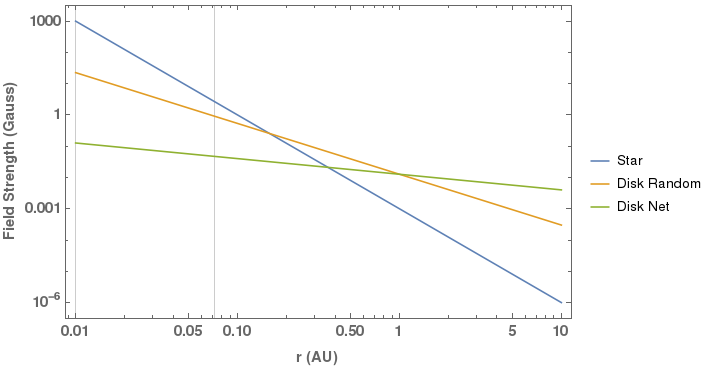
\includegraphics[width=0.8\columnwidth]{figs/figsChapter3/FieldStrengthProfiles.png}
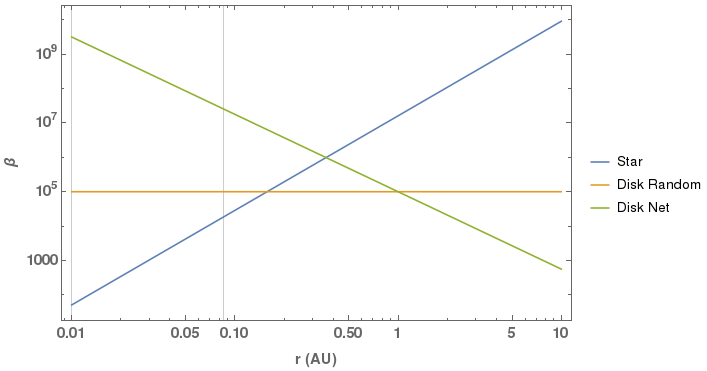
\includegraphics[width=0.8\columnwidth]{figs/figsChapter3/BetaProfiles.png}
\caption{Field strength profiles. Note: doesn't show all the things I claim it shows in the text yet.}
\label{fieldStrengthProfiles}
\end{figure}

The specific energy of the dipole field drops off faster than the gas pressure profile, meaning that the stellar magnetic field contribution will be dominant only in the inner part of the disk ($r<1$AU).  Magnetic field transport due to turbulence will make this region of influence larger, but only out to a few AU.

The stellar magnetic cycle causes the dipole field to vary in strength in a roughly sinusoidal way.  We will model this by adding flux to the disk during the positive-rising and negative-falling parts of the sine curve.  In the absence of transport, the flux added at each radii would be enough to make the net field of the disk equal to the stellar dipole strength at that radius after one quarter of a cycle (the duration of the positive-rising part of the sine curve).    




\newpage
\section{Location of the Ideal MHD to Hall MHD Transition}
The start of the dead zone occurs at the radius where the disk becomes too cool to be thermally ionized.  At this point the gas is in the Hall MHD regime and a Hall dead zone will exist.  This transition happens roughly at 800K.  Modeling the temperature profile of a disk is difficult, and different models can arrive at quite different profiles.  A large part of this uncertainty is due to the uncertainty in the dust fraction and distribution in the disk.  We will consider a variety of radii for the start of the Hall dead zone ranging from the inner boundary of the disk itself out to a few AU, with different cases being valid for different stellar masses and accretion rates.        

A simple active disk model with no incident radiation yields the temperature profiles shown in the following figure.  According to this model, only very quickly accreting disks would have a thermally ionized region at all (other disks will be truncated before 800K is reached).  However this model likely under-predicts temperature because it only accounts for one of the two major sources of heating: dissipation of the gravitational potential energy of accreting matter.  It does not consider radiation incident on the disk and does not account for vertical structure. 

The Chiang-Goldreich model is more sophisticated, accounting for incident radiation and dust.  Their model is only valid for $r>0.4$, but at this radius for a 0.5 solar mass star the model yields a temperature of about 220K, well below the 800K required for ionization.  So it's very reasonable to expect non-ideal MHD inside 1 AU for sub-solar-mass stars.  This also implies that in some situations the stellar dipole will contribute a dominant amount of net-flux directly into a Hall dead zone, not relying on transport within the disk for the flux to reach the dead zone.

\begin{figure}[p]
\centering
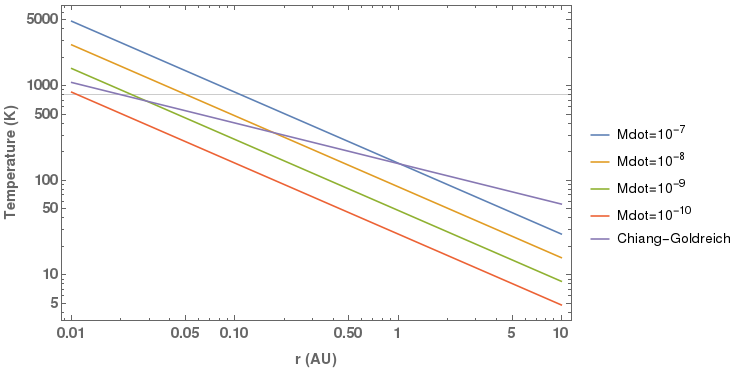
\includegraphics[width=0.8\columnwidth]{figs/figsChapter3/TemperatureProfiles.png}
\caption{Models of the temperature profile of an acitve disk around a sun-like star.}
\label{fiStExample}
\end{figure}

We will model the location of the start of the dead zone as static.  A more advanced model could dynamically calculate the location where $T=800$K and change the transport velocities accordingly, but this is difficult to do self consistently.  In addition, temperature by nature does not change as drastically as other quantities, so assuming this to be static is not completely unreasonable assumption.




\newpage
\section{A Simple Experiment: Turning the Dead Zone On and Off}
We will first consider a few simple test cases which will help us understand the more complicated cases later with the solar cycle turned on.  We will start with a roughly steady state net-field in the disk and then turn on the stellar dipole.  After half a cycle of driving (only in one direction), we will shut off the stellar dipole.  We will vary the polarity and strength of the initial and driving fields to demonstrate the relevant effects. 


\subsection{Stellar Dipole with the same Polarity as the Initial Disk Field}
These two cases are relatively straightforward diffusion, but the asymmetry between the two tests is important.  For the aligned disk field and aligned stellar dipole, the Hall DZ is in the active state and stays that way, so transport velocities are relatively high.  The additional field from the stellar dipole is transported outward smoothly and rather quickly to larger radii.  For the anti-aligned disk field and anti-aligned stellar dipole, the Hall DZ is in the dead state and remains that way.  This causes the transport velocities in this region to be much smaller than in the interior region.  The anti-aligned field contributed by the star is easily diffused to the inner edge of the DZ, but then builds up there as it makes it's way out into the DZ much more slowly.

\begin{figure}[p]
\centering
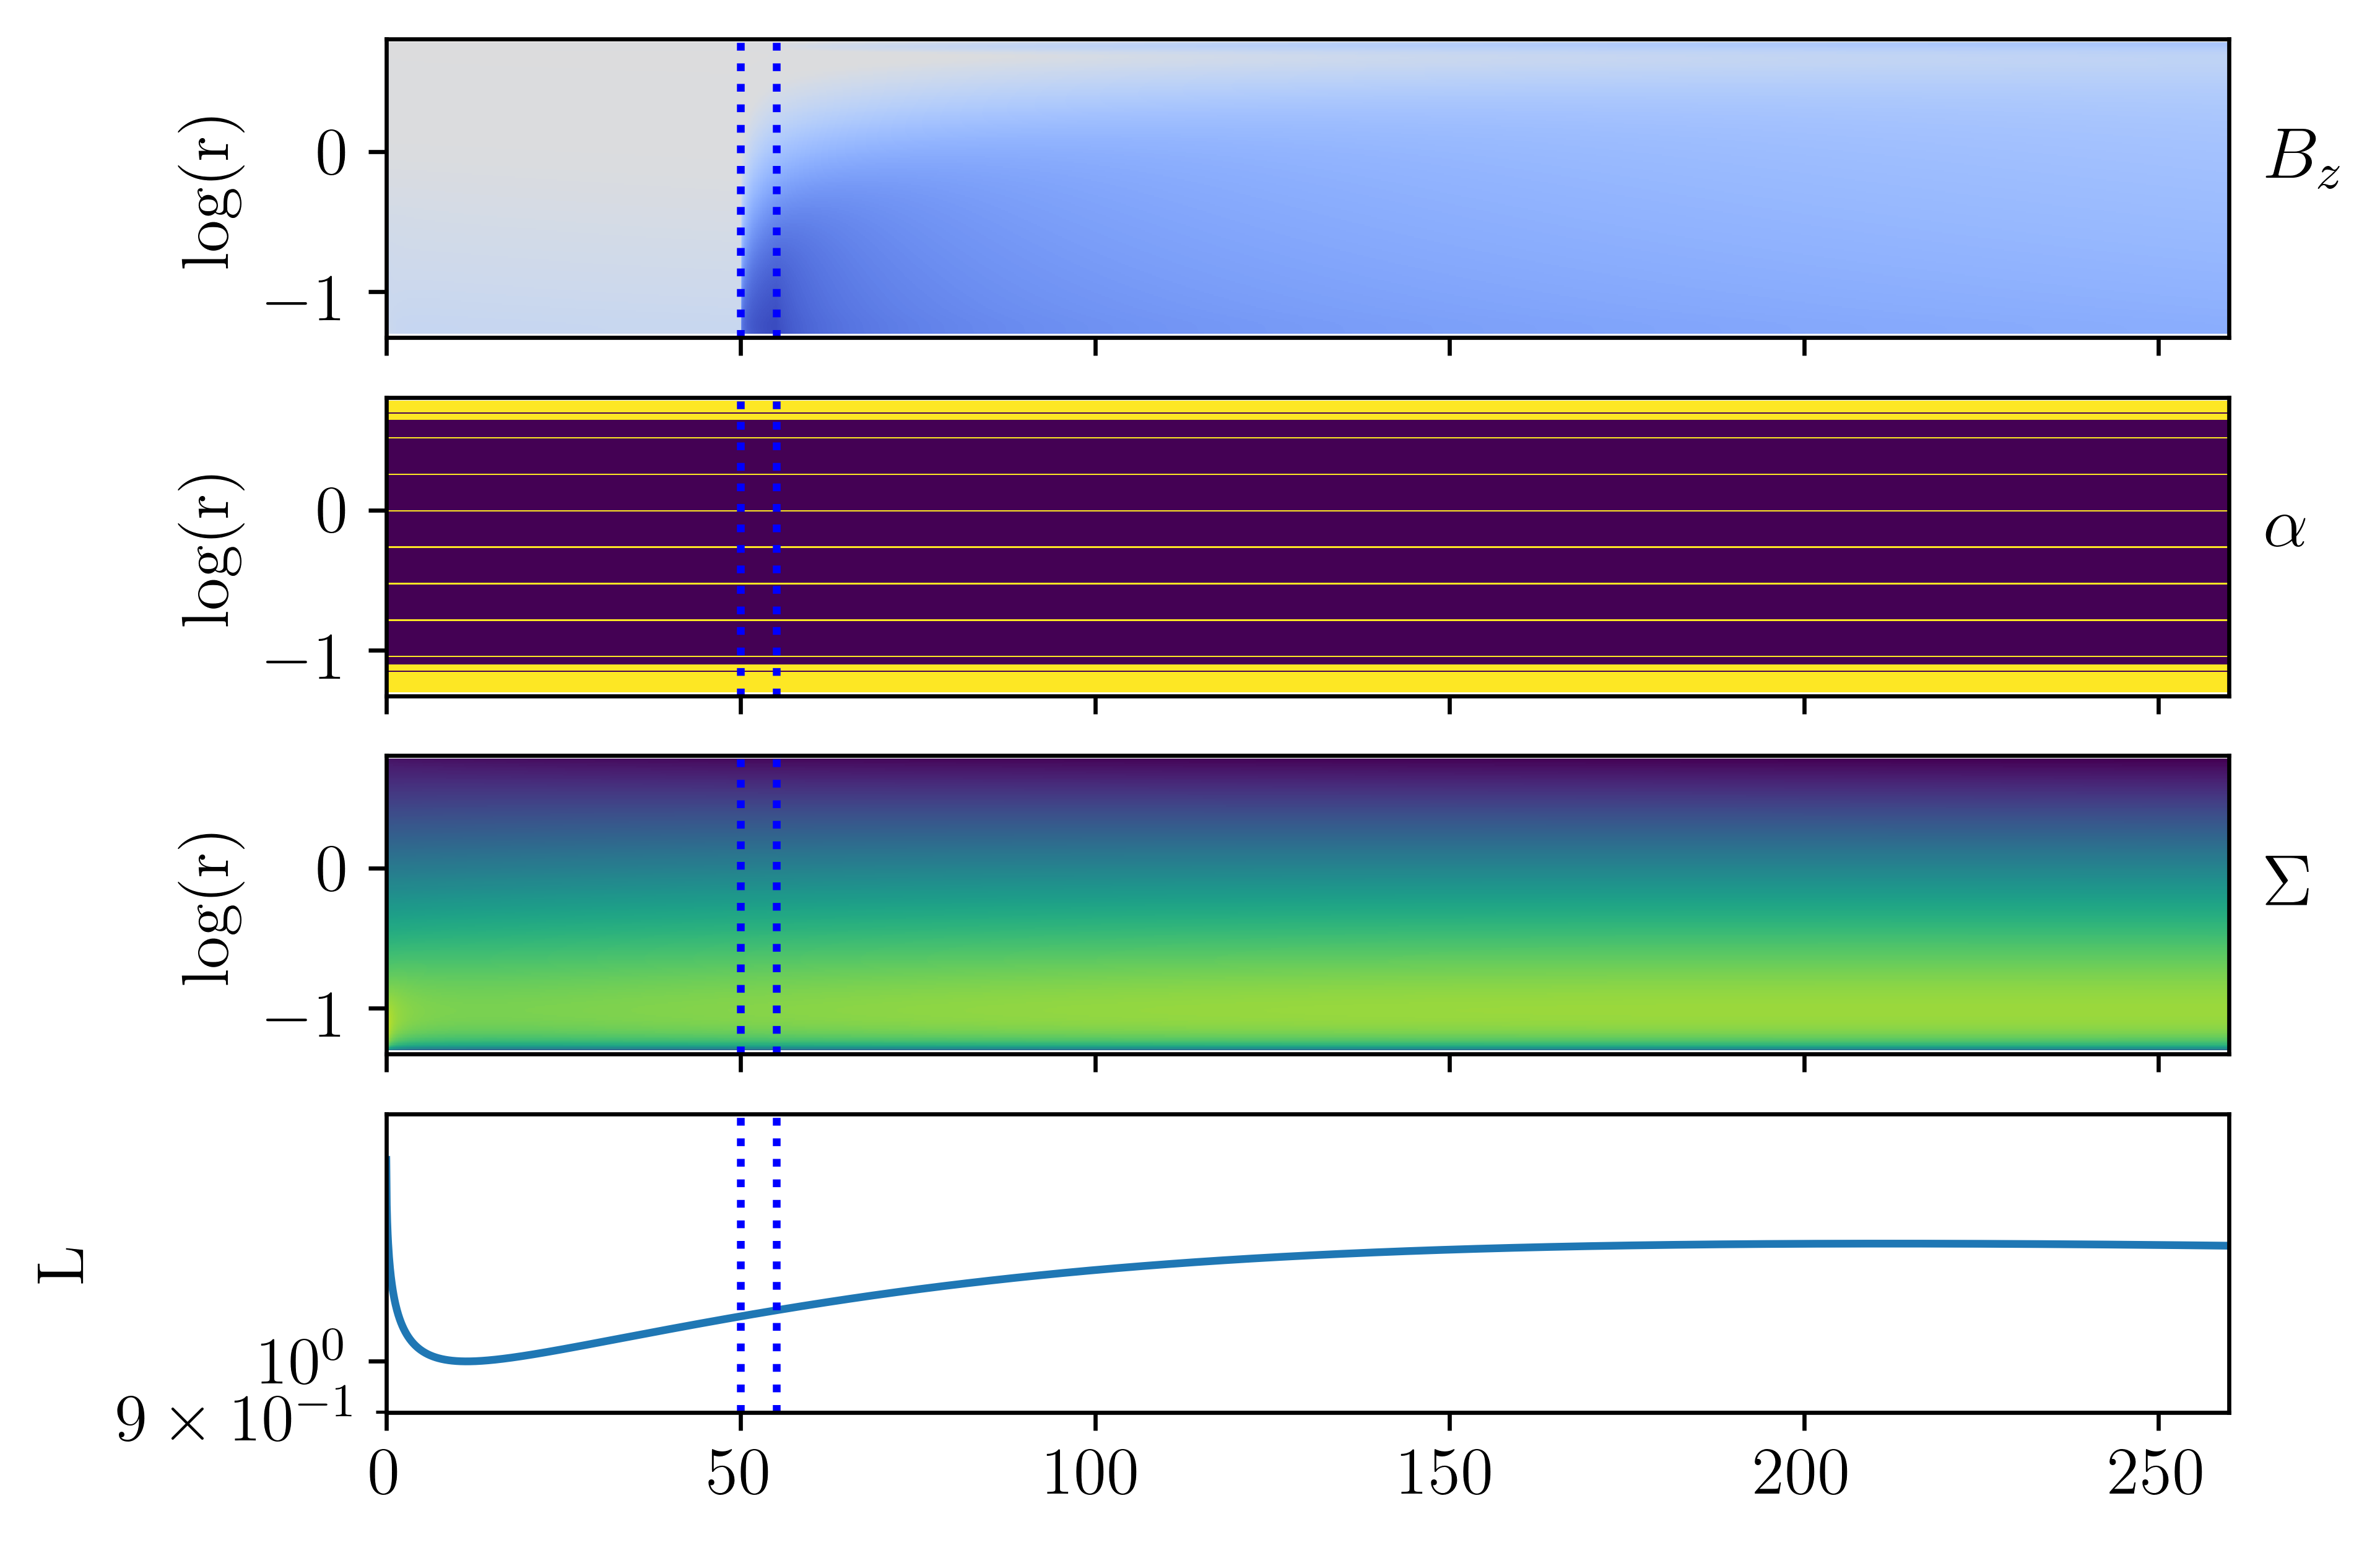
\includegraphics[width=0.7\columnwidth]{figs/figsChapter3/run3113/MST1.png}
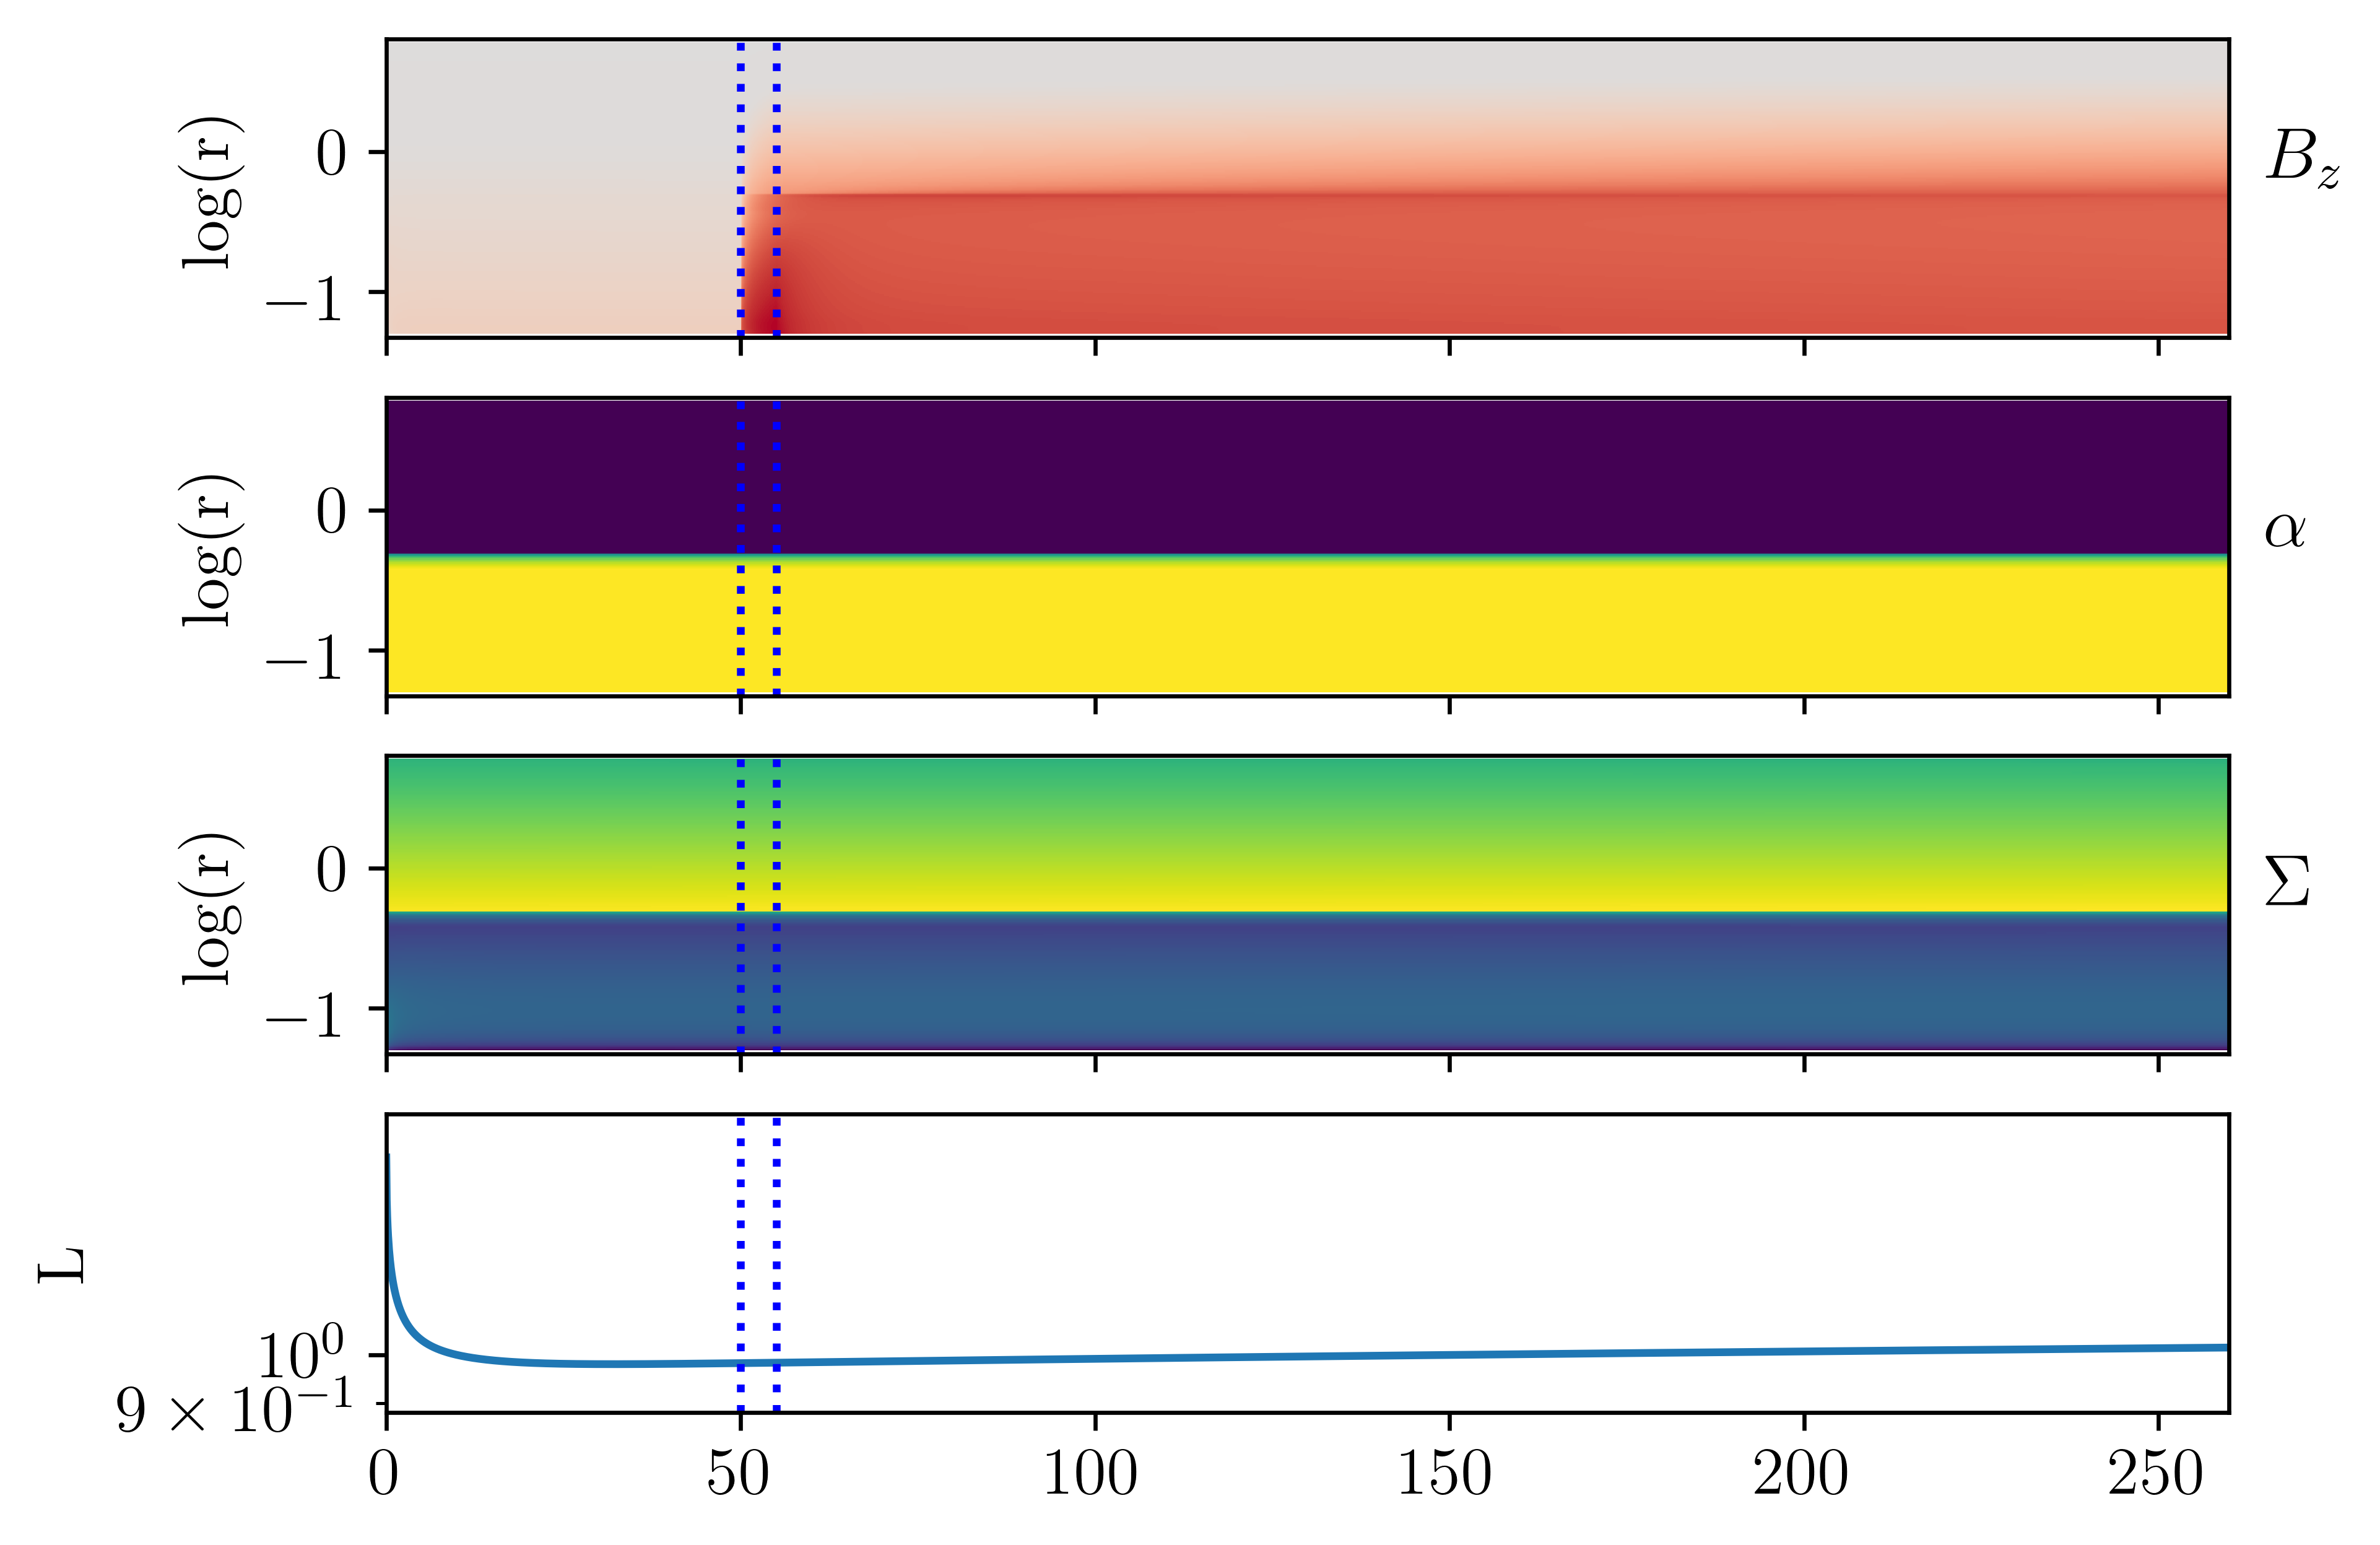
\includegraphics[width=0.7\columnwidth]{figs/figsChapter3/run3112/MST1.png}
\caption{}
\label{fiStExample}
\end{figure}

\newpage 
\subsection{Aligned Initial Field with Anti-Aligned Stellar Dipole}
In this case, the Hall DZ transitions from active to dead.  The extent of the Hall DZ that can be turned is limited primarily by 2 factors:
\begin{enumerate}
\item{The total amount of net-flux contributed to the disk by the stellar dipole relative to any already existing net-flux in the disk.}
\item{The amount of time that the field has to diffuse relative to the transport velocities in the disk.  It is important to note that these transport velocities are different in the active vs. dead state. }
\end{enumerate}
In our model, the stellar dipole contributes the same total amount of net flux to the disk regardless of the length of the stellar cycle.  The diffusion time and the accretion time are different, so it is likely that not all activated parts of the dead zone will be able to accrete all of their excess mass.

\begin{figure}[p]
\centering
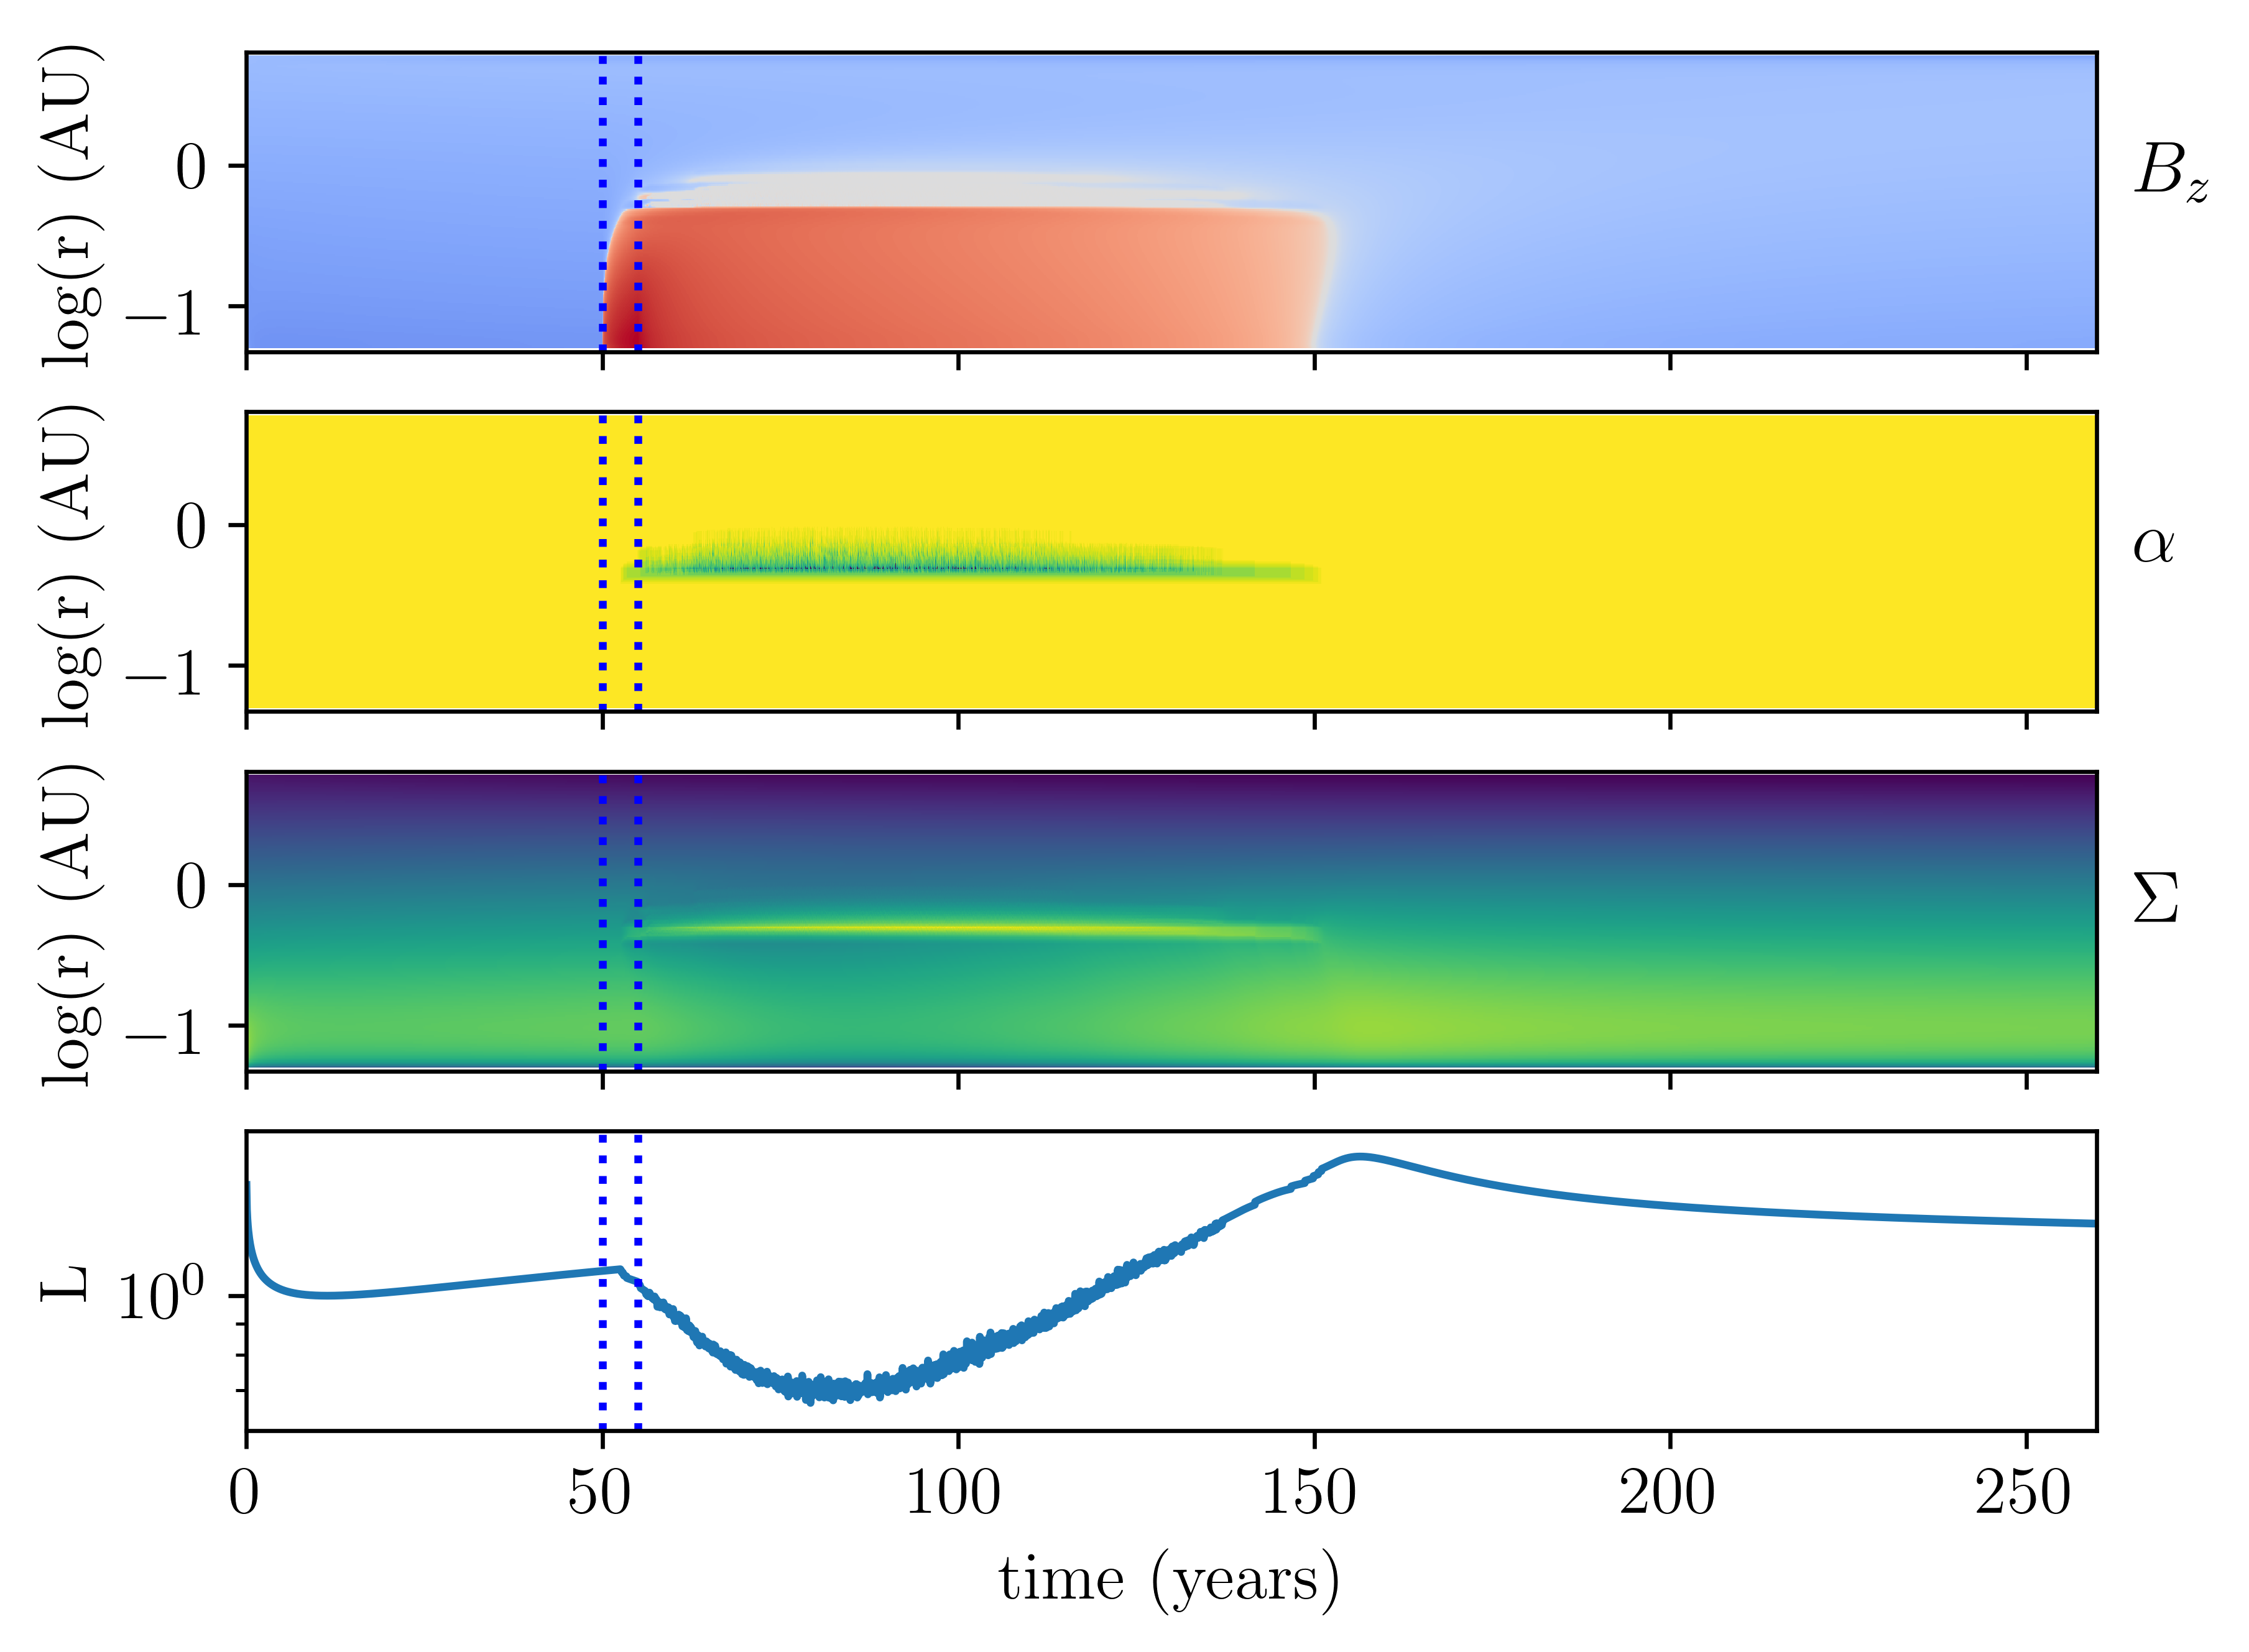
\includegraphics[width=0.7\columnwidth]{figs/figsChapter3/run3101/MST1.png}
\caption{The}
\label{fiStExample}
\end{figure}
 
\newpage
\subsection{Anti-Aligned Initial Field with Aligned Stellar Dipole}
 
\begin{figure}[p]
\centering
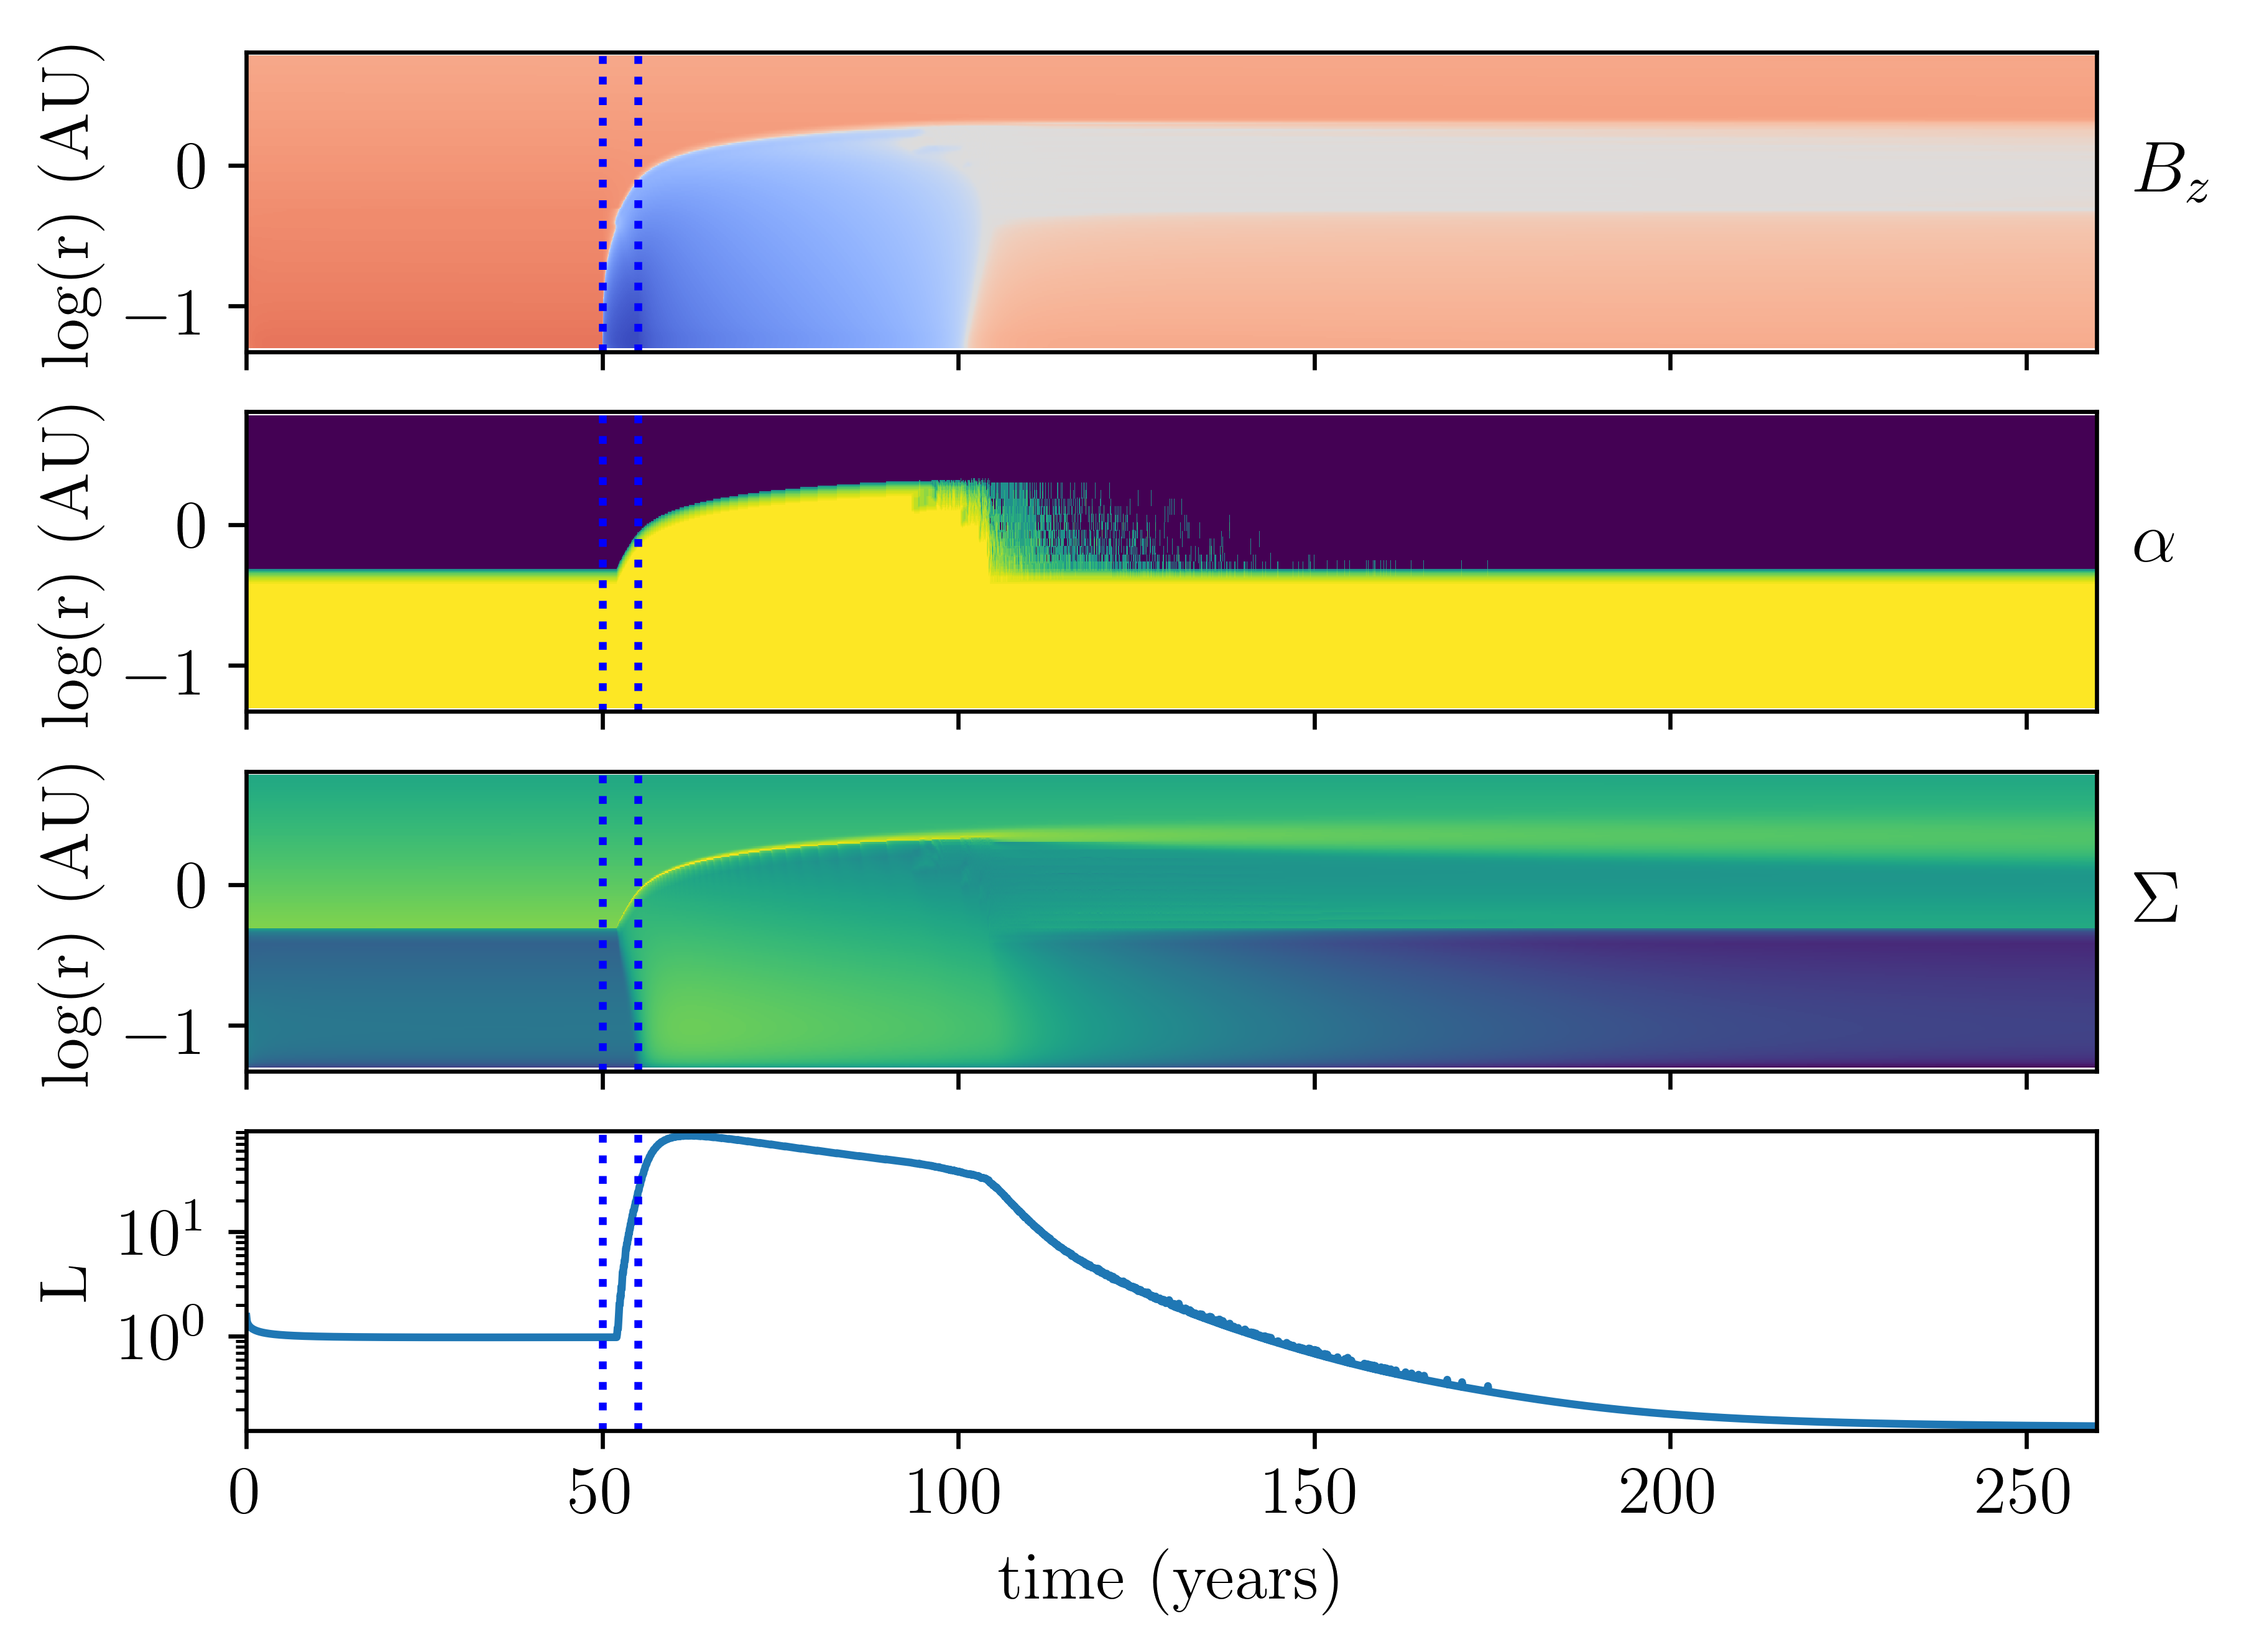
\includegraphics[width=0.7\columnwidth]{figs/figsChapter3/run3100/MST1.png}
\caption{The}
\label{fiStExample}
\end{figure}



 
\newpage
\section{A preference for Anti-Aligned Field}
Choosing the initial magnetic field is not obvious.  Is the DZ usually in the dead state with small bursts of activity caused by the stellar dipole oscillation?  Or is the DZ usually in the active state with intervening dead states caused by the stellar dipole oscillation?  We argue that, under the influence of the oscillating stellar dipole, the net magnetic field in the Hall DZ prefers to be in the anti-aligned direction such that the DZ is in the dead state, barring a strong field in the opposite direction that is inherent to the disk at formation.  This can be understood intuitively.  While in the dead state, net-field transport velocities are slow and the anti-aligned net-field is slow to diffuse away.  While in the active state, transport velocities are high and the aligned net-field is quick to diffuse away.  Due to this asymmetry in transport velocities, the DZ preferentially holds on to the anti-aligned field.

We will now demonstrate this numerically using our model.  The results of this test can be very biased by which direction we choose to start the stellar dipole.  In order to avoid this, we will start with a very weak dipole field that ramps up to more realistic values linearly over time.  Under these conditions the disk does not particularly care whether the dipole was initiated positive or negative.  The following figure shows that the stellar dipole field causes the field to eventually be in the anti-aligned direction as the dipole field strength ramps up.  Thus, in future calculations we will initialize the field with $B_z$ in the anti-aligned direction.    

\begin{figure}[p]
\centering
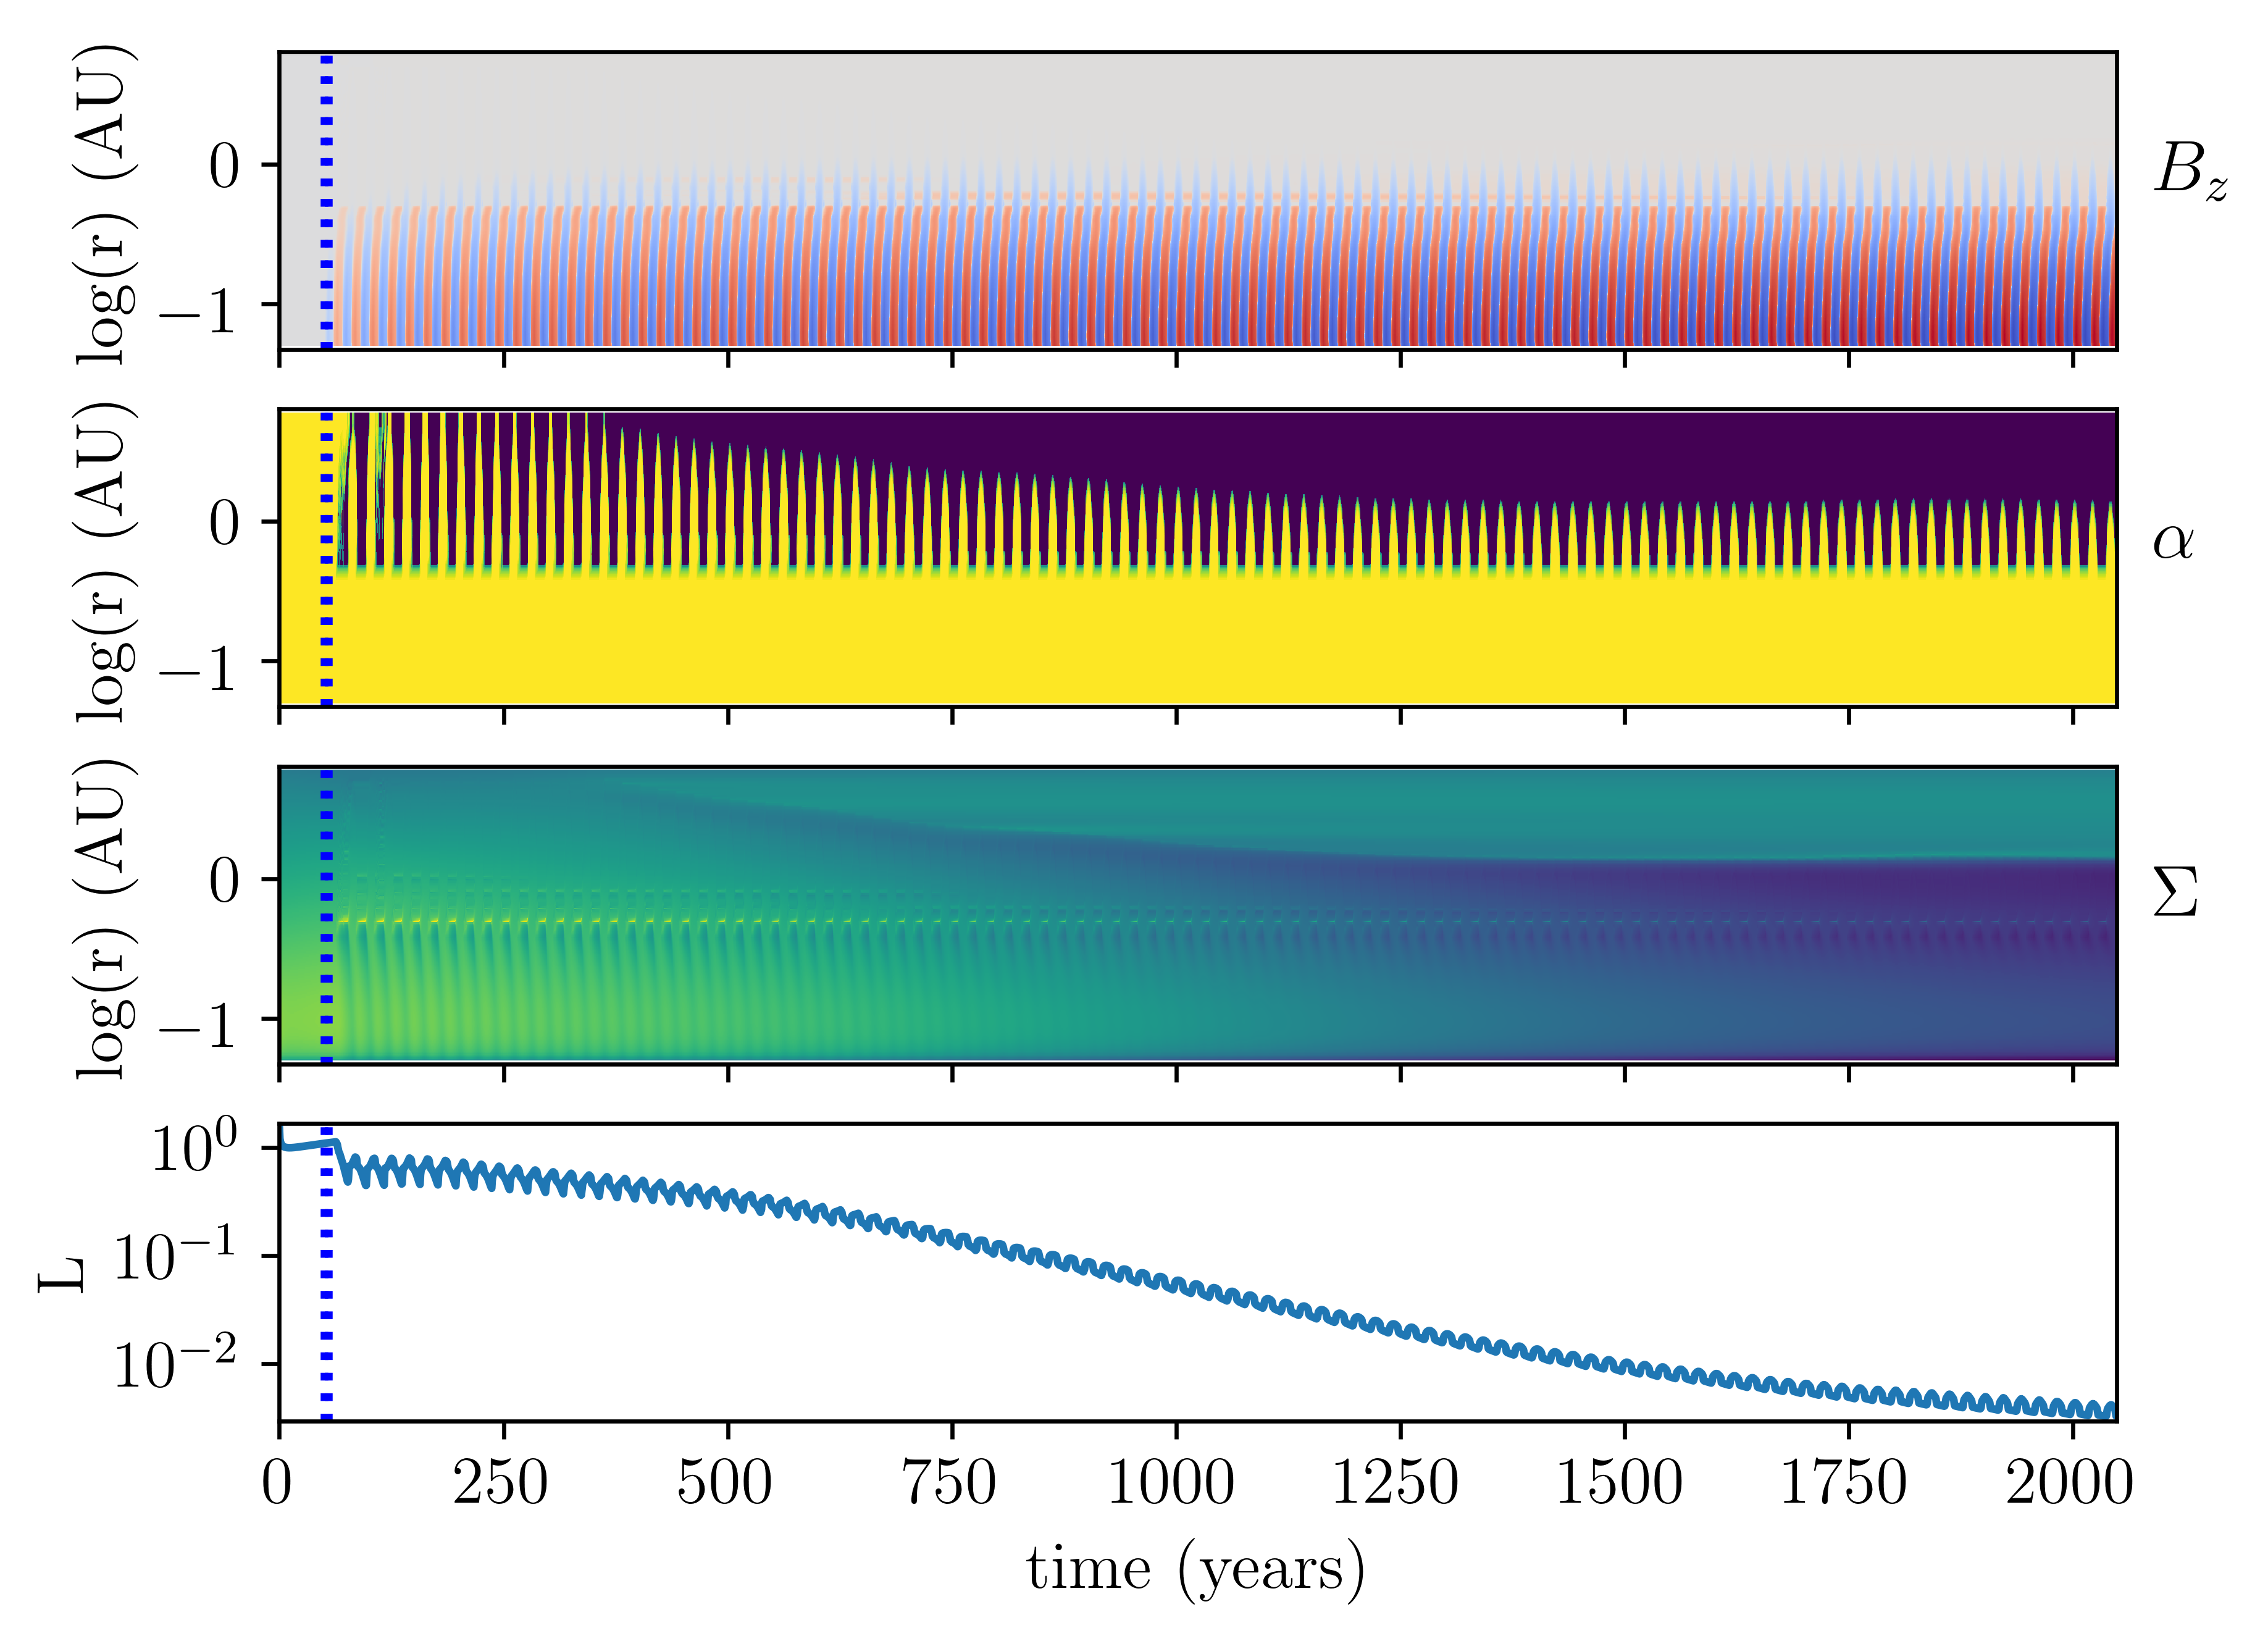
\includegraphics[width=0.7\columnwidth]{figs/figsChapter3/run3077/MST1.png}
\caption{The}
\label{fiStExample}
\end{figure}

 In order for $\dot{m}$ to be constant as a function of radius, the surface density in the dead zone must be enhanced by the same factor that the turbulent viscous transport is reduced.  This creates a large buildup of mass in the dead zone.  We will refer to this state as the "steady-fully-dead-state", in contrast to the "steady-fully-active-state", which has a flat $\alpha$ profile, and the usual (not piece-wise) power law profile for $\Sigma$.  We will use the term "excess mass" to refer to the enhancement in surface density in the dead zone for the steady-fully-dead-state compared to the steady-fully-active-state.   




\newpage
\section{Disks around small stars}
In this section we consider disks around small stars that will have no radii for which the mid-plane temperature exceeds 800K, and therefore will have a Hall dead zone all the way to the truncation radius.  This case is qualitatively different because the stellar dipole can contribute flux directly into the DZ without diffusion, although diffusion will still play a role.  

 
 
 
\newpage
\section{Flux Limited}
a




\newpage
\section{Observable Features and Comparison to Observed Phenomena}
a




\newpage
\section{Conclusions and Discussion}
We have modeled a mechanism that produces episodic accretion events in protoplanetary disks, similar in nature to observed EXors.  This mechanism is contingent on several features of these disks and their host stars:
\begin{enumerate}
\item{Hall dead zones exist in the inner disk ($\sim 0.1$ AU to $\sim 1$ AU) and suppress MRI turbulence only if the vertical magnetic field is anti-aligned with the spin axis. }
\item{The host star undergoes magnetic cycles in which the dipole-like field changes direction periodically.  This stellar field is able to leak into the very inner part of the disk ($\sim 0.01$ AU) significantly enough to dominate over any existing background field.}
\item{Thin disks efficiently diffuse magnetic field outward, allowing this stellar field to reach the Hall dead zone.}
\end{enumerate}

The qualitative features of the outbursts generated by this mechanism depend primarily on the time scale of the solar cycle relative to the diffusive and advective time-scales to the inner and outer edges of the Hall dead zone.  These time scales are determine by the scale height of the disc and the location and extent of the dead zone.

Several important conclusions:
\begin{enumerate}
\item{Hall dominated regions of the disk that are under the influence of a stellar magnetic cycle preferentially keep net magnetic field in the direction such that the dead zone is dead.}
\item{}
\item{}
\end{enumerate}
















